\documentclass[twocolumn,pra,aps,superscriptaddress]{revtex4-1}
\usepackage{xspace,amsmath,amsfonts,amsthm,amssymb,amsbsy, dsfont,graphics,color,graphicx,epsfig}
\usepackage{epstopdf,color}
%\usepackage[breaklinks=true]{hyperref}
\usepackage{relsize}
%\usepackage{url}
\usepackage{tikz}
\usetikzlibrary{decorations.text}
\usepackage{bm}
\usepackage{bbm}
\usepackage{listings}
% % \textwidth 16cm \textheight 23.5cm
% \renewcommand{\baselinestretch}{1.2}
\usepackage{graphicx}
\usepackage{graphics}
\usepackage{epsfig}
\usepackage{multirow}
%\usepackage[colorlinks]{hyperref}
\usepackage{fancyhdr}
\usepackage{calc}
\usepackage{natbib} %[numbers]
\usepackage{bibentry}
% underline tool
\usepackage[normalem]{ulem}
\usepackage[low-sup]{subdepth}
\usepackage{xcolor}
% triple lines in colors
\makeatletter
\newcommand\uuuline{\bgroup\markoverwith%
   {%
     \textcolor{red}{\rule[-0.5ex]{2pt}{0.4pt}}%
     \llap{\textcolor{blue}{\rule[-0.7ex]{2pt}{0.4pt}}}%
     \llap{\textcolor{green}{\rule[-0.9ex]{2pt}{0.4pt}}}%
   }%
   \ULon}
\makeatother

% todo list and commands
\usepackage{todonotes}
%% to avoid the conflict with amths package % not working
%\makeatletter
%\providecommand\@dotsep{5}
%\makeatother
%\listoftodos\relax
\usepackage{makeidx}
\allowdisplaybreaks

\newcommand{\sq}[1]{\left[ {#1} \right]}
\newcommand{\tr}[1]{{\textrm {Tr}}\sq{#1}}
\newcommand{\smallfrac}[2]{\mbox{$\frac{#1}{#2}$}}
\newcommand{\half}{\smallfrac{1}{2}}
\newcommand{\quarter}{\smallfrac{1}{4}}
\newcommand{\third}{\smallfrac{1}{3}}
\newcommand{\bra}[1]{\langle{#1}|}
\newcommand{\ket}[1]{|{#1}\rangle}
\newcommand{\braket}[2]{\langle{#1}|{#2}\rangle}
\newcommand{\ip}[2]{\langle{#1}|{#2}\rangle}
\newcommand{\op}[2]{\ket{#1}\!\bra{#2}}
\newcommand{\expt}[1]{\langle{#1}\rangle}
\newcommand{\dg}{^\dagger}
\newcommand{\red}{\color{red}}
\newcommand{\blue}{\color{blue}}
\newcommand{\cp}{\mathfrak{C}_p}


\begin{document}

\title{Don't forget names}
\author{Josh Combes, Adrian Chapman and Quanta}
\affiliation{Center for Quantum Information and Control, University of New Mexico, Albuquerque, NM 87131 USA}
\homepage{https://github.com/CQuIC/dont-forget-names}

\date{June 17 , 2017} % delete this line to display the current date
\begin{abstract}
\end{abstract}
\maketitle


%%% BEGIN DOCUMENT


\LARGE
% This part is the original part made by Josh Combes.
\begin{align}
A_\ell = \bar{e}\times \bar{a}_n \partial_r e
\end{align}

\begin{align}
\hat a\ket{n} = d\ket{y}
\end{align}

\begin{align}
B=\bar{e}\times \bar{n}
\end{align}

\begin{align}
C = \expt{a|\hat r| l}
\end{align}

\begin{align}
C + \det \left(\begin{array}{cc}h & s \\i & r\end{array}\right) = 0
\end{align}

\begin{align}
C = \frac{\hbar a} { r}  \op{l}{ i}_e
\end{align}

\begin{align}
I(\nu) = a\bar{\eta}
\end{align}

\begin{align}
\hat J_o = \hat S \hbar
\end{align}

\begin{align}
\frac{L}{e} = i g\hbar
\end{align}

\begin{align}
(MA)^\dag = T_IA\Sigma
\end{align}

\begin{align}
R\otimes B
\end{align}

\begin{align}
\hat S\ket{h} = (a_s\hbar + a_n)\ket{k}
\end{align}

\begin{align}
T_y = \ell\hat{e}_r/B_b^o
\end{align}

\begin{align}
V_i =c k/y
\end{align}

\begin{align}
Z(h) = -a_n g
\end{align}

% Below is the part made by Adrian Chapman, Ninnat Dangniam and others on Sep 3rd, 2015.
%\newpage
\begin{align}
\oint \vec{A} \cdot d \vec{r} &= i \vec{a} \cdot \vec{n}
\end{align}

\begin{align}
\hat{a}^{\dagger}_k i M \hat{a}_s \ket{a}
\end{align}

\begin{align} % Amir
\mathbf{AM} \ni IR
\end{align}

\begin{align} % Anirban
\left(\hat{a} \ket{n} \right)^{\dagger} i r  \hat{b} \hat{a} \ket{n}
\end{align}

\begin{align} %Ciaran
\sum c_i \bra{a} \hat{r} \ket{a}^n
\end{align}

\begin{align} %Elohim
\Sigma_{l} \hat{O} \hbar \ket{i, m}
\end{align}

\begin{align} % Ezad
\vec{E}(\vec{z}) = \tensor{\alpha} \cdot \vec{d}
\end{align}

\begin{align} %Gopi
G\left[\hat{O}, \hat{\rho}_i \right]
\end{align}

\begin{align}
j_0\left\vert n\right\rangle&=A^\mathsf{T}HA\left\vert n\right\rangle
\end{align}

\begin{align}
J = \frac{\partial (a, c)}{\partial (o, b)}
\end{align}

\begin{align}
\hat{K} = e^{i t \hat{H}}
\end{align}

\begin{align}
\mathbf{MA} \subseteq \mathbf{T}^{\mathbf{T}}
\end{align}

\begin{align}
\sum_{\mathlarger{n}} \braket{i}{n}\bra{n} a^{\dagger} \in T^*_o M
\end{align}

\begin{align} %Qi
\ket{q_i} &= \chi_i \, \tensor{\alpha}(0) \cdot \hat{\vec{d}}(0) \ket{n} \otimes \ket{g}
\end{align}

\begin{align} %Travis
\mathrm{Tr}\left(\hat{A}_\nu \hat{I} \right) = s
\end{align}

\begin{align} %Xijie
\chi_i = \vec{J}_{i} \cdot \vec{E}
\end{align}

\begin{align} %Zeke
Z = m c^2 + \frac{1}{2} m v^2
\end{align}

% The block for 2017.
\begin{equation} % Gloria
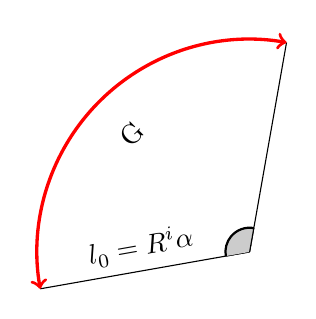
\begin{tikzpicture}[scale=1.5]
% Define variables.
\def\crad{1.8cm} 		% Radius of the big circle.
\def\arad{0.2cm} 	% Radius of the angle arc.
\def\sa{80}			% Starting angle of the angle arc.
\def\ea{190}		% Ending angle of the angle arc.
\coordinate (O) at (0,0);
%\coordinate (R) at (-0.07cm,0.71cm);
\coordinate (EP) at ([shift=(\ea:\arad)]0,0);
\coordinate (SP) at ([shift=(\sa:\arad)]0,0);
% Radius lines.
\draw (O) -- ++(\sa:\crad)
      (O) -- ++(\ea:\crad);
%\draw (R) node[rotate=-50] {$R^i$};
\path (EP) edge node[sloped,anchor=west,xshift=-1.2cm,above]{$l_0=R^i\alpha$} (O);
% Draw the big and small arcs which center at (0,0) with radius 1cm.
%\draw[thin,black]([shift=(\ea:\crad)]0,0) arc (\ea:(360+\sa):\crad);
\draw[very thick,red,<->] ([shift=(\sa:\crad)]0,0) arc (\sa:\ea:\crad); 
\path[sloped,decoration={text along path,reverse path,text={G},text align=center,raise=-0.7cm},decorate] ([shift=(\sa:\crad)]0,0) arc (\sa:\ea:\crad);
% Draw the short arc for the angle.
%\draw[very thick,black]([shift=(\sa:\arad)]0,0) node [left,black,yshift=0.08cm,rotate=-50]{$\alpha$} arc (\sa:\ea:\arad);
\draw[very thick,black]([shift=(\sa:\arad)]0,0) arc (\sa:\ea:\arad);
\filldraw[fill=black!20!white] (0,0) -- ([shift=(\sa:\arad)]0,0) arc (\sa:\ea:\arad) -- ([shift=(\ea:\arad)]0,0);
\end{tikzpicture}
\end{equation}


\end{document}

